\documentclass[]{beamer}
\usepackage[T1]{fontenc}
\usepackage[utf8]{inputenc}
\usepackage{lmodern}
\usepackage[italian]{babel}
\usepackage{mathrsfs}
\usepackage{cancel}

\title{Relatività}
\author{\texorpdfstring{Mattia Cozzi\newline\href{mailto:cozzimattia@gmail.com}{\texttt{cozzimattia@gmail.com}}}{Mattia Cozzi}}
\date{a.s.~2023/2024}

%\documentclass[handout]{beamer}     %usare questa classe per generare l'handout
%\usepackage{pgfpages}   %per mostrare più quadri nella stessa pagina
%\pgfpagesuselayout{4 on 1}[a4paper,border shrink=5mm,landscape]
\usetheme{Singapore}
%\useoutertheme[left]{sidebar} %elementi intorno alle diapositive
\setbeamercovered{dynamic} %modifica l'aspetto del testo grigetto delle diapositive future. Argomenti: invisible/transparent/dynamic
\usecolortheme{orchid}
%COLORE PRINCIPALE
% \definecolor{marroncino}{RGB}{156, 26, 0} % UBC Blue (primary)
% \setbeamercolor{structure}{fg=marroncino} % itemize, enumerate, etc


\theoremstyle{plain}
\newtheorem{teorema}{Teorema}

\usepackage{tikz}
\usepackage{circuitikz}


\usepackage{pgf,pgfplots,graphicx}
\usetikzlibrary{angles,quotes,arrows,shapes,decorations.markings}
\pgfplotsset{compat=1.15}
\usepgfplotslibrary{units,fillbetween} % to add units easily to axis
\tikzset{fleche/.style args={#1:#2}{postaction=decorate,decoration={name=markings,mark=at position #1 with {\arrow[#2,scale=2]{>}}},},}


\def\angolo[#1](#2)(#3:#4:#5)% Syntax: [draw options] (center) (initial angle:final angle:radius)
    { \draw[#1] ($(#2)+({#5*cos(#3)},{#5*sin(#3)})$) arc (#3:#4:#5); }

\begin{document}

\begin{frame}
  \titlepage
\end{frame}





\begin{frame}
\frametitle{Contenuti}
\tableofcontents
\end{frame}

%slide sull'invarianza della velocità della luce

\section{M{\&}M}



\begin{frame}
\frametitle{Contesto storico}
\begin{columns}
\begin{column}{0.2\textwidth}
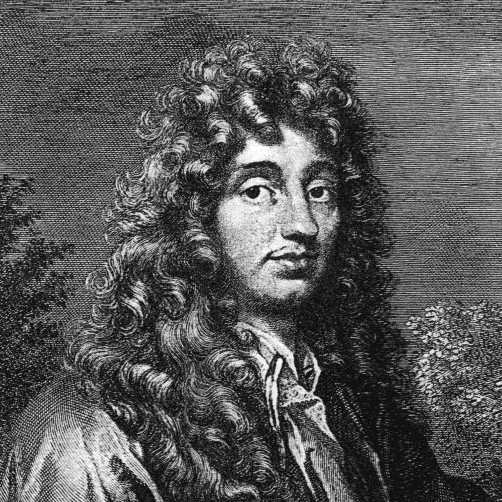
\includegraphics[width=\columnwidth]{img/huygens.jpg}

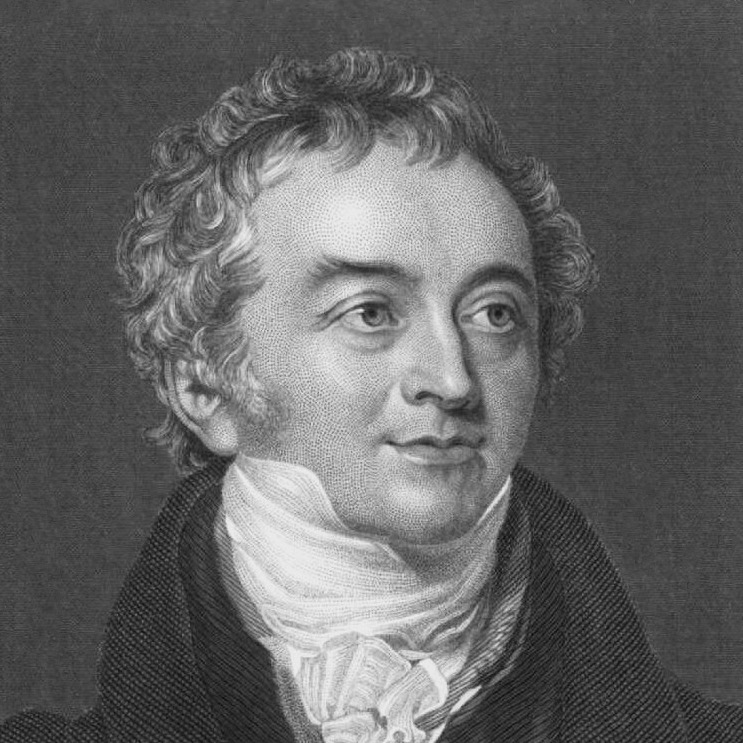
\includegraphics[width=\columnwidth]{img/young.jpg}

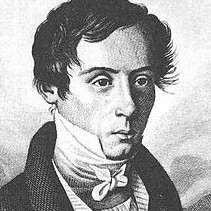
\includegraphics[width=\columnwidth]{img/fresnel.jpg}
\end{column}
\begin{column}{0.7\textwidth}
Nel 1678 \alert<1>{Huygens} formula una \emph{teoria ondulatoria della luce}, estesa poi da \alert<1>{Young} e \alert<1>{Fresnel} nel XIX secolo.\pause

\begin{small}
\begin{itemize}
\item<2-> la luce è intesa come un'onda che si propaga in un mezzo (l'\alert<2>{etere luminifero}, Young 1804) formato da particelle elastiche e che permea tutto l'universo;
\item<3-> nel XIX secolo la teoria di Huygens, grazie agli esperimenti su \alert<3>{interferenza} e \alert<3>{diffrazione}, è preferita a quella corpuscolare (Descartes 1637 e Newton 1672).
\end{itemize}
\end{small}
\end{column}
\end{columns}
\end{frame}


%approfondimento sulle varie misurazioni della velocità della luce EVITABILE!!!!

\begin{frame}
  \frametitle{Il ruolo dell'etere luminifero}
  L'esistenza dell'etere luminifero permetterebbe di spiegare la contraddizione tra meccanica classica ed elettromagnetismo.\pause
  
  Potremmo infatti affermare che:
  \begin{block}{Validità delle equazioni di Maxwell}
    le equazioni di Maxwell sono valide solo nel SDR in cui l'etere è in quiete
  \end{block}
e poiché la Terra è in moto nello spazio, l'etere sulla Terra non è in quiete.
\end{frame}


\begin{frame}
  \frametitle{Il vento d'etere (1)}
  Per verificare l'ipotesi occorre rilevare con un esperimento l'esistenza del ``vento d'etere'', il moto della Terra nell'etere in quiete.\pause
  
  L'esperimento venne proposto dallo stesso Maxwell già nel 1875 quando scrisse la voce \emph{Ether} per l'\emph{Encyclop\ae dia Britannica}. \href{https://tinyurl.com/y3bbs8kg}{\beamergotobutton{Link all'articolo}}\\~\\  
  \begin{quote}
    {\small Se fosse possibile determinare la velocità della luce, osservando il tempo che impiega per viaggiare tra una stazione e un'altra sulla superficie della Terra, potremmo, confrontando le velocità osservate in direzioni opposte, determinare la velocità dell'etere rispetto a queste stazioni terrestri.}
  \end{quote}
\end{frame}


\begin{frame}
  \frametitle{Il vento d'etere (2)}
  Poiché la Terra si muove con una certa velocità, può essere considerata ferma e investita da un vento di etere con pari velocità, ma diretto in senso contrario al moto della Terra.
  \begin{figure}
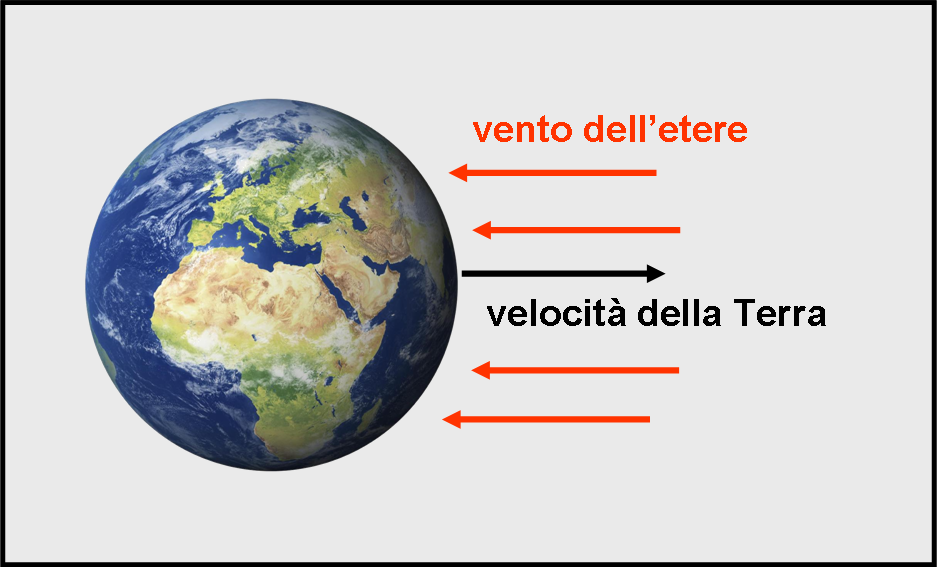
\includegraphics[width=.6\columnwidth]{img/etere.png}    
  \end{figure}
    Se esiste l'etere, allora i raggi luminosi devono subire l’effetto dell’etere.
\end{frame}

\begin{frame}
  \frametitle{Il vento d'etere (3)}
  \begin{columns}
    \begin{column}{0.5\textwidth}
      \begin{figure}
        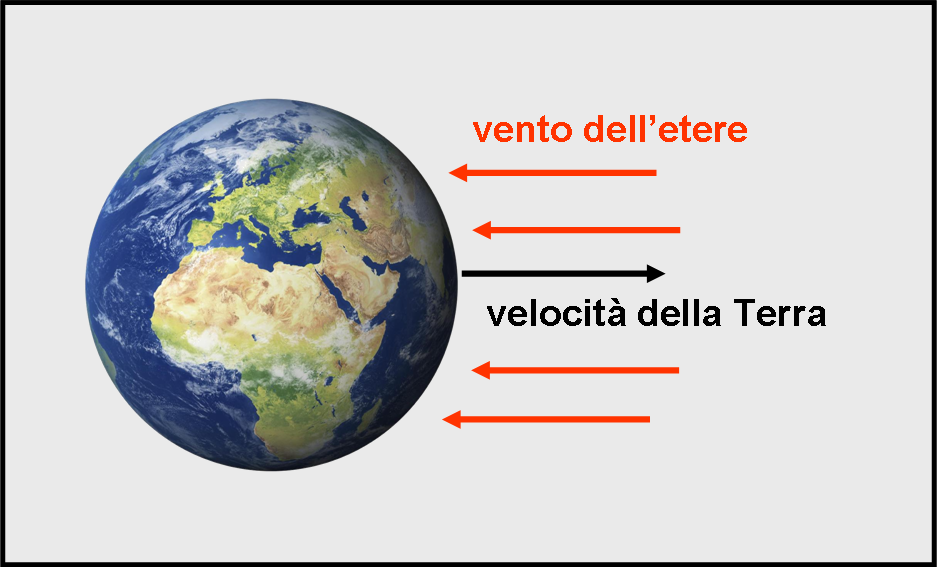
\includegraphics[width=\columnwidth]{img/etere.png}
      \end{figure}
    \end{column}
    \begin{column}{0.5\textwidth}
      \begin{figure}
        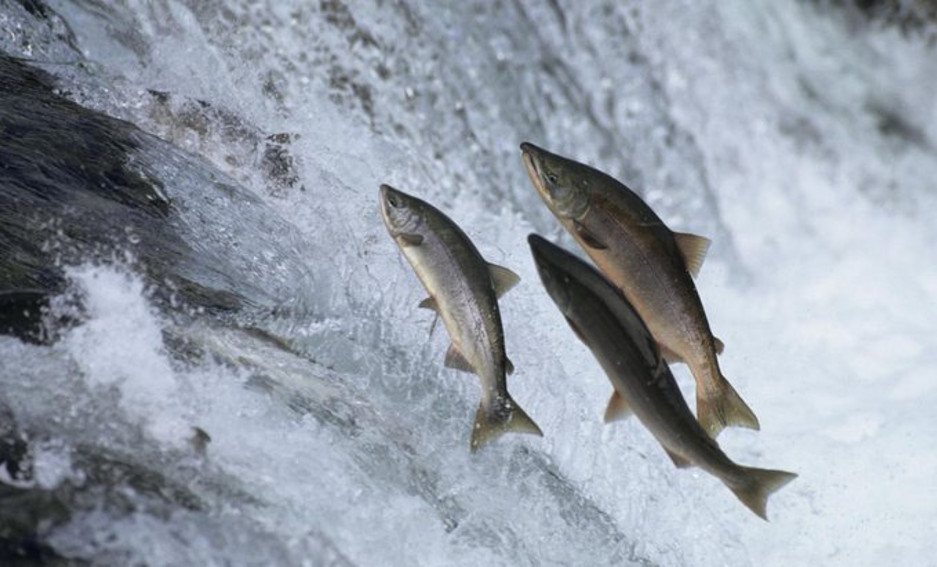
\includegraphics[width=\columnwidth]{img/salmone.jpg}
      \end{figure}
    \end{column}
  \end{columns}
  ~\\~\\Se le onde luminose viaggiano nella direzione del moto della Terra saranno investite dal vento dell’etere e troveranno un po' di resistenza, se invece viaggiano in senso contrario saranno aiutate nella loro corsa.
\end{frame}

\begin{frame}
\frametitle{L'esperimento di Michelson-Morley}
Il problema principale è la enorme velocità della luce, che impedisce una misurazione diretta. Il genio di Michelson nel 1881 (e poi con maggior precisione con Morley nel 1887) fu usare la lunghezza d'onda come misura indiretta del tempo che un raggio luminoso impiega a percorrere un tratto rettilineo, sfruttando cioè il fenomeno dell'\alert<1>{interferenza}.\\~\pause\\

Si fanno percorre a dei raggi luminosi percorsi di eguale lunghezza ma con orientamenti diversi (rispetto al vento d'etere). I raggi luminosi, essendo sospinti o rallentati dal vento d'etere, dovrebbero percorrere tali percorsi in \alert<2>{tempi diversi}.\\~\pause\\

I raggi vengono poi convogliati su uno schermo per mostrarne la \alert<3>{figura di interferenza}.
\end{frame}


\begin{frame}
  \frametitle{Risultato dell'esperimento}
I risultati mostrano che, anche cambiando l'orientamento dei percorsi effettuati dai raggi luminosi, la figura d'interferenza rimane sempre identica, falsificando l'ipotesi del vento d'etere.
  \begin{columns}
    \begin{column}{0.3\textwidth}
      \begin{figure}
        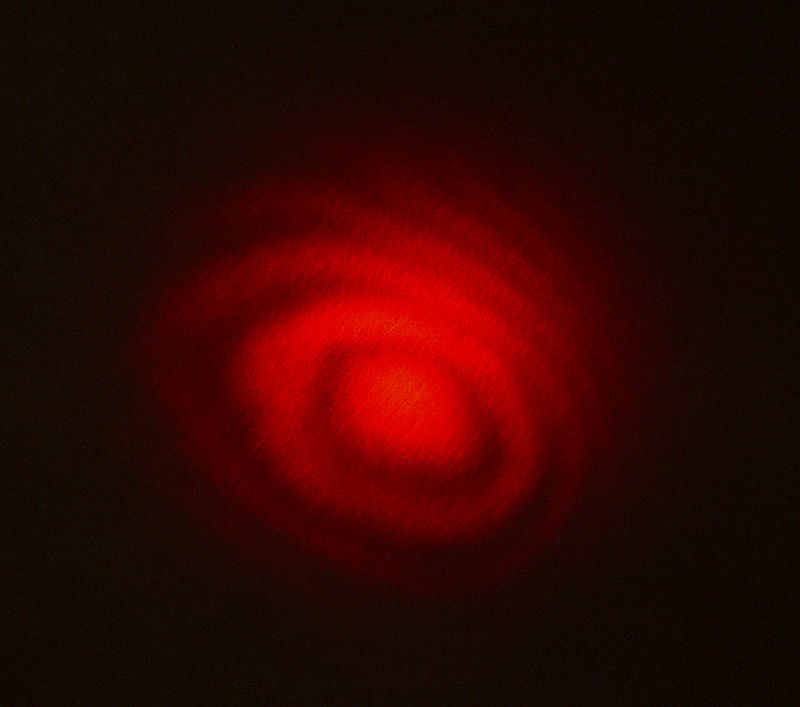
\includegraphics[width=\columnwidth]{img/figuramorley.jpg}
        
        {\footnotesize Interferenza dei raggi ``spinti'' dall'etere}
      \end{figure}
    \end{column}
    \begin{column}{0.3\textwidth}
      \begin{figure}
        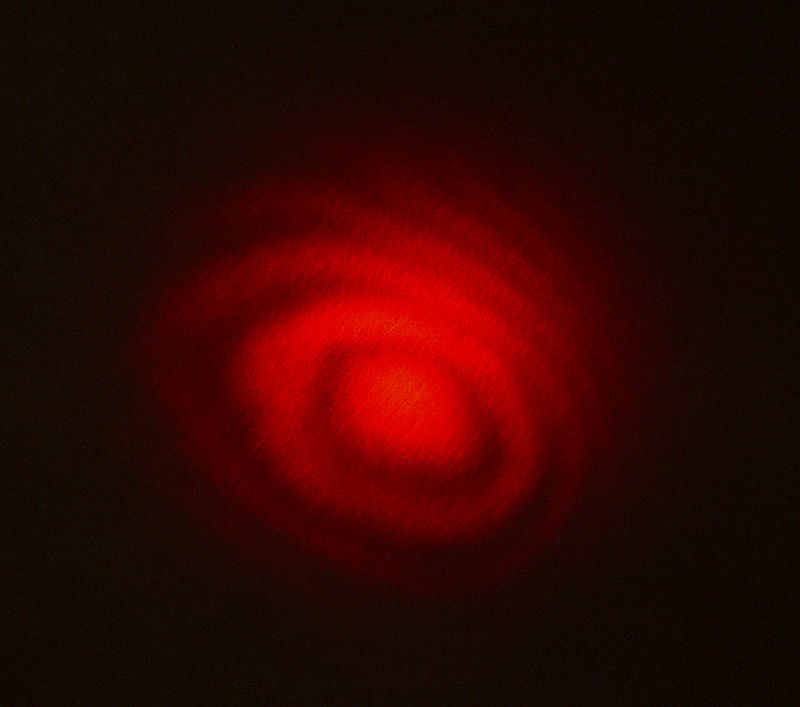
\includegraphics[width=\columnwidth]{img/figuramorley.jpg}
        
        {\footnotesize Interferenza dei raggi ``frenati'' dall'etere}
      \end{figure}
    \end{column}
  \end{columns}
\end{frame}


\begin{frame}
  \frametitle{Ulteriori riferimenti}
  Due ottimi articoli sull'esperimento di Michelson e Morley:\\~\\
  
\begin{center}
  \href{http://www.infinitoteatrodelcosmo.it/2017/10/09/la-favola-michelson-dei-due-fotoni-soluzione-del-quiz-sul-nobel/}{\beamergotobutton{LA FAVOLA DI MICHELSON E DEI DUE FOTONI}}\\~\\
  
  \href{http://www.infinitoteatrodelcosmo.it/2017/10/16/la-scomparsa-delletere-michelson-ad-einstein/}{\beamergotobutton{LA SCOMPARSA DELL’ETERE: DA MICHELSON AD EINSTEIN}}
\end{center}
\end{frame}

\section{Einstein}

\begin{frame}
\frametitle{Contesto}
\begin{columns}
\begin{column}{0.2\textwidth}
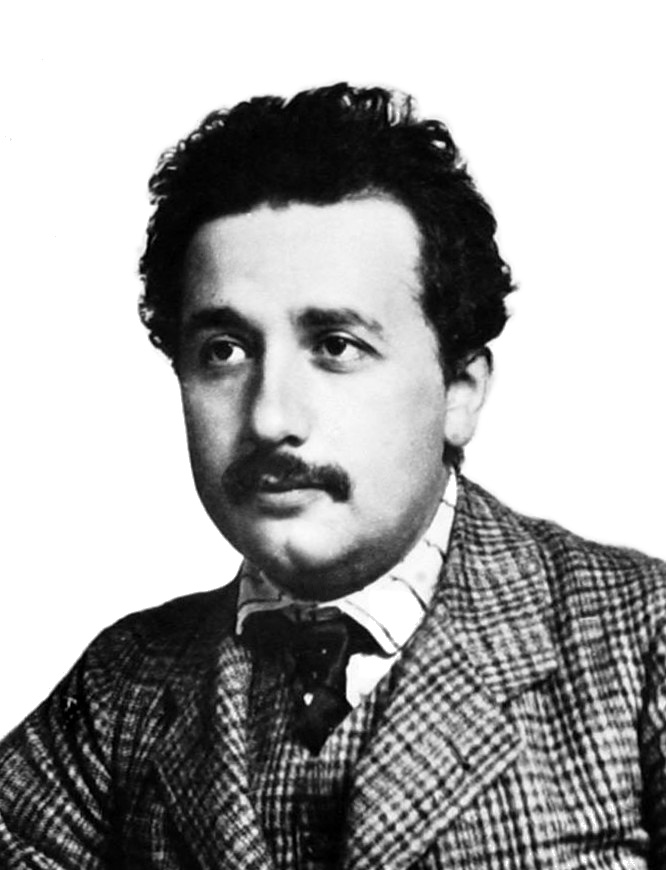
\includegraphics[width=\columnwidth]{img/einstein.jpg}
\end{column}
\begin{column}{0.7\textwidth}
\begin{center}
  1905
\end{center}
\emph{Annus mirabilis} di Einstein, che pubblica quattro articoli fondamentali:\pause

\begin{small}
\begin{enumerate}
\item<2-> studia l'effetto fotoelettrico, ipotizzando la \alert<2>{doppia natura della luce};
\item<3-> analizza il moto browniano, contribuendo ad affermare l'\alert<3>{ipotesi atomica della materia};
\item<4-> propone la \alert<4>{relatività ristretta} pur senza conoscere il risultato di M\&M, ma spinto da ragioni di semplicità ed eleganza formale;
\item<5-> dimostra l'equivalenza tra massa ed energia: \alert<5>{$ E=mc^2 $}.
\end{enumerate}
\end{small}
\end{column}
\end{columns}
\end{frame}





\begin{frame}
\frametitle{Assiomi della relatività ristretta}
La contraddizione restava aperta e fu affrontata da Einstein proponendo una rifondazione della fisica sulla base di \alert<1>{due assiomi}:\pause
\begin{block}{Principio di relatività ristretta\footnote{Estensione del principio di relatività galileiana, che vale solo per la meccanica.}}
  Le leggi e i principi della fisica hanno la stessa forma in tutti i sistemi di riferimento inerziali.
\end{block}\pause
\begin{block}{Principio di invarianza di $ c $}
La velocità della luce è la stessa in tutti i sistemi di riferimento inerziali, indipendentemente dal moto del sistema stesso o della sorgente da cui la luce è emessa\footnote{Spiega il risultato di Michelson e Morley.}.
\end{block}
\end{frame}



\begin{frame}
  \frametitle{Tempo assoluto?}
  Einstein parte dalla messa in discussione di un fatto che fino ad allora era stato dato per scontato: che il tempo scorresse \alert<1>{identico in ogni sistema di riferimento}, un tempo assoluto.\\~\pause\\In effetti, nelle trasformazioni di Galileo, vale $ t = t' $.\\~\pause\\  
  La critica di Einstein al tempo assoluto parte dal concetto di \alert<3>{simultaneità}.
\end{frame}







\section{Simultaneità}

\begin{frame}
\frametitle{Simultaneità di due eventi (1)}
Parliamo di simultaneità di due eventi quando essi si verificano nello stesso momento.\\~\pause\\

Ordinariamente, se si accendono simultaneamente due lampadine poste alla stessa distanza da noi, la loro luce deve raggiungerci nel medesimo istante: \alert<2-3>{$ A \rightarrow B $}.\\~\pause\\
Possiamo inoltre dire che se la luce di due lampadine poste alla stessa distanza ci raggiunge nello stesso istante, i due eventi luminosi devono essere stati simultanei: \alert<3>{$ B \rightarrow A $}, e quindi \alert<3>{$ A \leftrightarrow B $}.
\end{frame}

\begin{frame}
\frametitle{Simultaneità di due eventi (2)}
Questo tuttavia accade nella vita di tutti i giorni, quando le velocità considerate sono molto inferiori a $ c $.\\~\pause\\

In realtà la simultaneità è un fenomeno che \alert<2>{dipende dal sistema di riferimento}. Cominciamo fornendo una \emph{definizione operativa\footnote{Una definizione operativa indica gli strumenti di misura e la procedura del loro utilizzo.} di simultaneità} sulla base dell'assioma di invarianza di $ c $.
\end{frame}

\begin{frame}
  \frametitle{Definizione operativa di simultaneità}
  Immaginiamo due fenomeni (emissioni di luce) $ F_1 $ e $ F_2 $ che si verificano nei punti $ A $ e $ B $, equidistanti da un rilevatore posto nel punto $ C $. Definiamo che:
  \begin{block}{Simultaneità}
  I due fenomeni $ F_1 $ e $ F_2 $ sono simultanei se la luce che emettono giunge nello stesso istante in un punto equidistante da essi.
  \end{block}  
\begin{figure}
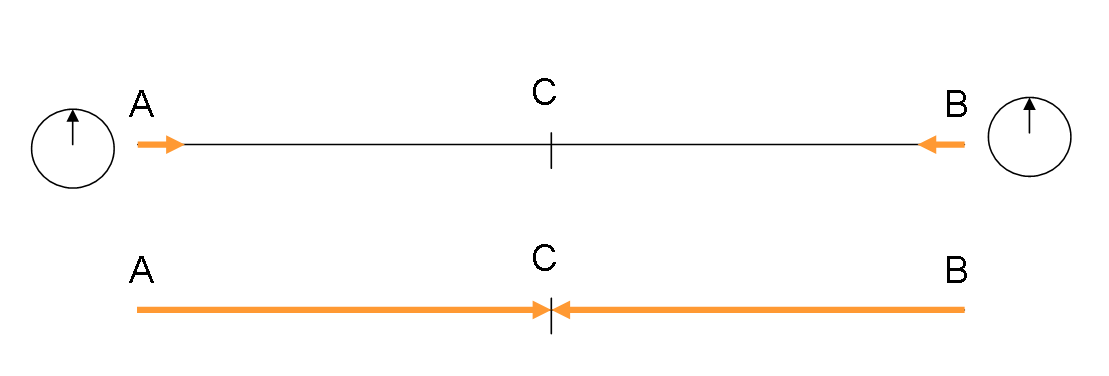
\includegraphics[width=.6\columnwidth]{img/simultaneita.png}
\end{figure}
\end{frame}




\begin{frame}
  \frametitle{Simultaneità e SDR (1)}
La definizione operativa appena fornita porta a risultati ``inaspettati'' se applicata a rilevatori che si muovono l'uno rispetto all'altro (l'esempio è dello stesso Einstein).\\~\pause\\

Immaginiamo due osservatori:
\begin{itemize}
  \item $ O_1 $ posto a terra, equidistante dai punti $ A $ e $ B $.
  \item $ O_2 $ posto su un treno in moto verso $ O_1 $;
\end{itemize}~\pause\\
Immaginiamo che quando $ O_2 $ passa davanti a $ O_1 $ due lampadine si accendano nei punti $ A $ e $ B $ e che la loro luce viaggi in tutte le direzioni con velocità $ c $, identica in ogni SDR.
\end{frame}


\begin{frame}
  \frametitle{Simultaneità e SDR (2)}
Dalla definizione operativa appena data, risulta che $ O_1 $ valuterà che i due fenomeni sono stati \emph{simultanei} (egli è equidistante da $ A $ e $ B $ e la luce percorre la stessa distanza nello stesso tempo).\\~\pause\\
$ O_2 $ valuterà invece i due eventi come \emph{non simultanei}, poiché nel tempo impiegato dalla luce a raggiungerlo, il treno si è spostato e la luce dovrà percorrere distanze diverse alla medesima velocità (finita), impiegando quindi tempi diversi.\\~\pause\\Il giudizio di simultaneità è relativo (al SDR)!
\end{frame}


\begin{frame}
  \frametitle{Sincronizzazione degli orologi}
  Proviamo allora a confrontare la durata di un eventi in SDR diversi. Per poterlo fare, dobbiamo disporre di \emph<1>{orologi sincronizzati}.\\~\pause\\Per due orologi posti a distanza $ D $:
  \begin{block}{Orologi sincronizzati}
    Due orologi sono sincronizzati se il secondo di essi, nell'istante in cui riceve un lampo di luce emesso dal primo al tempo $ t $ segna il tempo: \begin{center}
    $ t' = t + \dfrac{D}{c} $
    \end{center}
  \end{block}
\end{frame}


\section{Dilatazione}


\begin{frame}
  \frametitle{Apparato sperimentale (1)}
  Vogliamo misurare la durata del raggio luminoso emesso da un orologio posto su un carrello mobile. Il raggio viene emesso, riflesso da uno specchio, e rilevato dall'orologio dopo un certo tempo.\\~\pause\\Immaginiamo due osservatori diversi:
  \begin{itemize}
    \item $ O_1 $ a terra (SDR$ _1 $);
    \item $ O_2 $ sul carrello in moto con velocità $ \vec{v} $ rispetto a $ O_1 $ (SDR$ _2 $).
  \end{itemize}
\end{frame}

\begin{frame}
  \frametitle{Apparato sperimentale (2)}
\begin{columns}
\begin{column}{0.4\textwidth}
\visible<1->{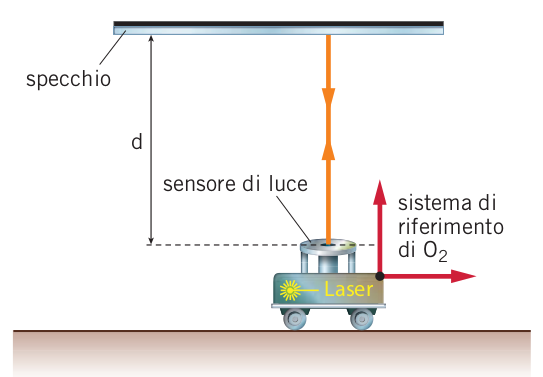
\includegraphics[width=\columnwidth]{img/dilatazionetempi1.png}}

~

~

\visible<2>{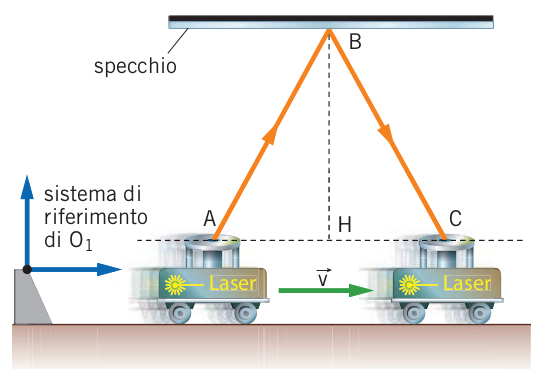
\includegraphics[width=\columnwidth]{img/dilatazionetempi2.png}}
\end{column}
\begin{column}{0.6\textwidth}
\begin{footnotesize}
~\\~\\~\\
\visible<1->{Poiché $ v = \dfrac{\Delta s}{\Delta t} $, allora nel sistema di riferimento di $ O_2 $:
\begin{center}
$ \Delta t = \dfrac{2d}{c} $
\end{center}}
~\\~\\~\\
\visible<2>{Nel SDR$ _1 $ il raggio segue una traiettoria diversa e valgono le seguenti relazioni:
\begin{center}
$ \overline{AB} = \dfrac{1}{2} c\Delta t' $~~~~$ \overline{HB} = \dfrac{1}{2} c\Delta t $\\~\\$ \overline{AH} = \dfrac{1}{2} v\Delta t' $
\end{center}
oltre al teorema di Pitagora su $ ABH $.}
\end{footnotesize}
\end{column}
\end{columns}
\end{frame}


\begin{frame}
  \frametitle{Risultati}
  Inserendo le relazioni valide nel SDR$ _2 $ nella formula del teorema di Pitagora, otteniamo:
  \begin{center}
  $ c^2 (\Delta t')^2 = v^2 (\Delta t')^2 + c^2 (\Delta t)^2 $
  \end{center}
  da cui, isolando $ \Delta t' $:\pause
  \begin{center}
  \colorbox{blue!30}{$ \Delta t' = \dfrac{1}{\sqrt{1- \left( \dfrac{v}{c} \right)^2 }}\Delta t $}
  \end{center}
  che mostra che i due intervalli di tempo, misurati in due SDR diversi, non sono uguali!
\end{frame}




\begin{frame}
  \frametitle{Dilatazione dei tempi}
\begin{small}
    \begin{center}
$ \Delta t' = \dfrac{1}{\sqrt{1- \left( \frac{v}{c} \right)^2 }}\Delta t $
  \end{center}
  \end{small}
  Essendo $ v \leq c $, il denominatore della formula precedente è sempre minore o uguale a 1, e pertanto $ \Delta t' \geq \Delta t $.\\~\pause
  \begin{block}{Dilatazione di tempi}
    La durata di un fenomeno è minima quando essa è misurata in un SDR solidale con il baricentro del sistema fisico in esame\footnote{Da qui il ``paradosso dei gemelli''.}.
  \end{block}\pause~\\
  La durata del fenomeno misura in un sistema solidale con esso è detta \alert{intervallo di tempo proprio $ \Delta \tau $}.
\end{frame}


\begin{frame}
  \frametitle{$ \beta $ e $ \gamma $}
  Definiamo \colorbox{blue!30}{$ \beta = \dfrac{v}{c} $} ($ \beta \leq 1 $){\pause} e pertanto:
\begin{center}
  \colorbox{blue!30}{$ \gamma = \dfrac{1}{\sqrt{1- \left( \frac{v}{c} \right)^2 }} = \dfrac{1}{\sqrt{1 - \beta^2}} $}
\end{center}
{\pause}e scriveremo semplicemente:
  \begin{center}
  \colorbox{blue!30}{$ \Delta t' = \gamma\Delta t $}
  \end{center}
  $ \gamma $ è detto \alert{fattore di Lorentz}.
\end{frame}


\begin{frame}
  \frametitle{Il fattore di Lorentz (1)}
  Possiamo leggere nel fattore $ \beta = \dfrac{v}{c} $ la percentuale della velocità della luce alla quale avviene il moto nel SDR considerato.{\pause}\\~\\  
  Ad esempio, se $ v = 1 \times 10^8 \, \frac{m}{s} $:
  \begin{center}
  $ \beta = \dfrac{1 \times 10^8 \, \frac{m}{s}}{3 \times 10^8 \, \frac{m}{s}} = \dfrac{1}{3} = 0,\overline{3} \approx 33 \% $
  \end{center}
  {\pause}
  Studiamo l'andamento di $ \gamma $ al variare di $ v $.
\end{frame}




\begin{frame}
  \frametitle{Il fattore di Lorentz (2)}
  
  
  \begin{columns}
\begin{column}{0.4\textwidth}

\scriptsize 
    \centering
  \begin{tabular}{c|c|c}
    $ \mathbf{\beta} $ & $ \mathbf{\gamma} $ & $ \mathbf{\gamma}^{-1} $\\\hline\rule{0pt}{3ex}
    $ 0,010 $ & $ 1,000 $ & $ 1,000 $ \\\rule{0pt}{3ex}
    $ 0,100 $ & $ 1,005 $ & $ 0,995 $ \\\rule{0pt}{3ex}
    $ 0,200 $ & $ 1,021 $ & $ 0,980 $ \\\rule{0pt}{3ex}
    $ 0,300 $ & $ 1,048 $ & $ 0,954 $ \\\rule{0pt}{3ex}
    $ 0,400 $ & $ 1,091 $ & $ 0,917 $ \\\rule{0pt}{3ex}
    $ 0,500 $ & $ 1,155 $ & $ 0,866 $ \\\rule{0pt}{3ex}
    $ 0,600 $ & $ 1,250 $ & $ 0,800 $ \\\rule{0pt}{3ex}
    $ 0,700 $ & $ 1,400 $ & $ 0,714 $ \\\rule{0pt}{3ex}
    $ 0,800 $ & $ 1,667 $ & $ 0,600 $ \\\rule{0pt}{3ex}
    $ 0,866 $ & $ 2,000 $ & $ 0,500 $ \\\rule{0pt}{3ex}
    $ 0,900 $ & $ 2,294 $ & $ 0,436 $ \\\rule{0pt}{3ex}
    $ 0,990 $ & $ 7,089 $ & $ 0,141 $ \\\rule{0pt}{3ex}
    $ 0,999 $ & $ 22,366 $ & $ 0,045 $ \\
  \end{tabular}

\end{column}
\begin{column}{0.6\textwidth}
\begin{figure}
\begin{tikzpicture}[xscale=1.4,yscale=.4]
\draw [->] (-.15,0) -- (3.5,0);
\draw [->] (0,-.5) -- (0,9);
\draw [dotted] (0.5,0) -- (0.5,1);
\draw [dotted] (1,0) -- (1,1.1);
\draw [dotted] (1.5,0) -- (1.5,1.2);
\draw [dotted] (2,0) -- (2,1.4);
\draw [dotted] (2.5,0) -- (2.5,1.8);
\draw [dotted] (3,0) -- (3,7.8);
\draw[smooth, orange, thick, domain=0:2.99, samples=50] plot 
({\x},{    (1- (.11*\x^2))^-.5           });
\node [below] at (.5,0) {{\tiny $ 0,5 $}};
\node [below] at (1,0) {{\tiny $ 1 $}};
\node [below] at (1.5,0) {{\tiny $ 1,5 $}};
\node [below] at (2,0) {{\tiny $ 2 $}};
\node [below] at (2.5,0) {{\tiny $ 2,5 $}};
\node [below] at (3,0) {{\tiny $ 3 $}};
\node [below] at (1.5,-1.5) {{\tiny $ v \, (\times 10^8 \, \frac{m}{s}) $}};
\node [left] at (0,1) {{\tiny $ 1 $}};
\node [left] at (0,2) {{\tiny $ 2 $}};
\node [left] at (0,3) {{\tiny $ 3 $}};
\node [left] at (0,4) {{\tiny $ 4 $}};
\node [left] at (0,5) {{\tiny $ 5 $}};
\node [left] at (0,6) {{\tiny $ 6 $}};
\node [left] at (0,7) {{\tiny $ 7 $}};
\node [left] at (0,8) {{\tiny $ 8 $}};
\node [left] at (-.3,4.5) {{\tiny $ \gamma $}};
\end{tikzpicture}

~

\footnotesize
$ \displaystyle \lim_{v \to c} \frac{1}{\sqrt{1- \left( \frac{v}{c} \right)^2 }} = + \infty  $

\end{figure}
\end{column}
\end{columns}
\end{frame}





\begin{frame}
\frametitle{Esercizi}
\begin{exampleblock}{Calcolo della velocità (1)}
\small{
  Anche i processi biologici devono soddisfare gli assiomi della relatività.

  Quale velocità deve avere una navicella perché il suo equipaggio invecchi della metà rispetto al personale di controllo rimasto a terra? Esprimi il risultato con due cifre significative in funzione di $ c $.\hspace*{\fill}[$ 0,87c $]
  }
\end{exampleblock}

~

\begin{exampleblock}{Utilizzo delle percentuali}
\small{
  Nel sistema di riferimento in moto l'intervallo di tempo misurato supera del $ 10\% $ il suo tempo proprio.
  
  Qual è la velocità di un osservatore rispetto all'altro?\hspace*{\fill}[$ \pm 0,417c $]
  }
\end{exampleblock}
\end{frame}




\section{Contrazione}

\begin{frame}
  \frametitle{Apparato sperimentale (1)}
Immaginiamo di nuovo un treno che si muove a velocità $ v $ e due osservatori: $ O_1 $ a terra e $ O_2 $ sul treno.\\~\\
Vogliamo misurare la \alert<1>{lunghezza $ \Delta x $} di un segmento $ \overline{AB} $ posto al suolo e \alert<1>{parallelo alla direzione del treno}.\\~\pause\\
\alert<2>{Per $ O_1 $ la posizione di $ A $ e $ B $ è costante nel tempo} e, se il treno impiega un tempo $ \Delta t $ per passare da $ A $ a $ B $, vale:
\begin{center}
\colorbox{blue!30}{$ \Delta x = v \Delta t $}
\end{center}
\end{frame}


\begin{frame}
  \frametitle{Apparato sperimentale (2)}
  \alert<1>{Per $ O_2 $} la situazione è più complessa, perché nel suo SDR \alert<1>{$ \overline{AB} $ è in movimento a velocità $ v $}.\\~\pause\\  
  $ O_2 $ valuterà la lunghezza di $ \overline{AB} $ misurando il \alert<2>{tempo $ \Delta t' $ necessario affinché prima il punto $ A $ e poi il punto $ B $ passino per un certo punto $ P $ del treno} (ad esempio davanti a lui).\\~\pause\\  
  Poiché per $ O_2 $ gli estremi del segmento si muovono a velocità $ v $, vale:
\begin{center}
\colorbox{blue!30}{$ \Delta x' = v \Delta t' $}
\end{center}
\end{frame}


\begin{frame}
  \frametitle{Risultati (1)}
Notiamo tuttavia che il passaggio di $ A $ e $ B $ per $ P $ è un evento solidale con il SDR$ _2 $ e quindi \alert<1>{$ \Delta t' $ è il tempo proprio dell'evento} ed è sempre più breve di $ \Delta t $. Vale pertanto:
\begin{center}
$ \Delta t = \gamma \Delta t' $~~~ e quindi ~~~$ \Delta t' = \dfrac{\Delta t}{\gamma} $
\end{center}
Sapendo che $ \Delta x = v \Delta t $ e $ \Delta x' = v \Delta t' $ otteniamo:
\begin{center}
$ \Delta x' = v \Delta t' = v \dfrac{\Delta t}{\gamma} = \dfrac{(v \Delta t)}{\gamma} = \dfrac{\Delta x}{\gamma} $
\end{center}
\end{frame}


\begin{frame}
  \frametitle{Risultati (2)}
  \begin{center}
\colorbox{blue!30}{$ \Delta x' = \dfrac{\Delta x}{\gamma} $}
\end{center}\pause
\begin{block}{Contrazione delle lunghezze}
La lunghezza di un segmento misurata in un SDR in moto rispetto ad esso è sempre minore della lunghezza misurata nel SDR in cui esso è in quiete.
\end{block}~\pause\\    
La lunghezza del un segmento misurata nel SDR in cui esso è in quiete è detta \alert{lunghezza propria} e risulta la maggiore possibile.
\end{frame}

\begin{frame}
  \frametitle{Lunghezze parallele e perpendicolari}
  \begin{alertblock}{Attenzione!}
    La contrazione delle lunghezze è un fenomeno che si verifica solo per lunghezze \emph{parallele} alla velocità del segmento, mentre le lunghezze \emph{perpendicolari} alla velocità risultano inalterate.
  \end{alertblock}
\end{frame}





\begin{frame}
\frametitle{Esercizi}
\begin{exampleblock}{Calcolo della velocità (2)}
\small{
  Un'asta rigida è lunga $ 2,00 \, m $ misurata nel sistema di riferimento ad essa solidale.

Con quale velocità deve muoversi rispetto ad un osservatore perché gli appaia contratta di $ 1,00 \, m $?
  }
\end{exampleblock}

~

\begin{exampleblock}{Lunghezze parallele e perpendicolari}
\small{
  Un oggetto ha una forma circolare, di raggio $ r = 32 \, cm $, quando è fermo. In moto rettilineo uniforme alla velocità di $ 2,0 \times 10^{5} \, km/s $ rispetto a un osservatore fermo al suolo, l'oggetto apparirebbe di forma diversa.
  \begin{itemize}
    \item Dimostra che l'oggetto circolare, una volta in moto, appare ellittico.
    \item Calcola la lunghezza degli assi dell'ellisse nel SDR dell'osservatore.\hspace*{\fill}[$ 64 \, cm $, $ 48 \, cm $]
  \end{itemize}
  }
\end{exampleblock}
\end{frame}




\section{Lorentz}
\begin{frame}
  \frametitle{Le trasformazioni di Galileo}
  La meccanica newtoniana utilizza le trasformazioni di Galileo per descrivere un fenomeno in due SDR diversi.\\~\pause\\    
  Supponiamo due SDR in moto relativo a velocità $ v $ lungo l'asse $ x $:
    \[
  \left\{ 
  \begin{array}{l}
  x' = x - vt; \quad\quad y' = y; \quad\quad z' = z;\\
  t' = t
  \end{array}
  \right. 
  \]\pause
  Tali trasformazioni non prendono in considerazione gli effetti relativistici e devono quindi essere modificate opportunamente.
\end{frame}


\begin{frame}
  \frametitle{Le trasformazioni di Lorentz}
Furono proposte a fine XIX secolo da diversi fisici (tra cui Hendrik Lorentz) come trasformazioni sotto le quali le equazioni di Maxwell rimangono invarianti passando da un SDR ad un altro.\\~\pause\\
Se prendiamo come direzione dell'asse $ x $ in entrambi i SDR la direzione del vettore $ \vec{v} $, avranno forma:

\begin{center}
\colorbox{blue!30}{$ \left\{ 
  \begin{array}{l}
  x' = \gamma (x - vt);\\
  y'=y;\\
  z'=z;\\
  t' = \gamma \left( t - \dfrac{\beta}{c^2}x \right).
  \end{array}
  \right.   $}

~
  
~

\href{https://www.youtube.com/watch?v=Rh0pYtQG5wI}{\beamergotobutton{Video: visualizzare le trasformazioni di Lorentz}}
\end{center}

\end{frame}


\begin{frame}
  \frametitle{Galileo come caso particolare}
  Per velocità molto inferiori a $ c $, \alert{$ \beta \approx 0 $} e \alert{$ \gamma\approx 1 $}, e vediamo come le trasformazioni di Lorentz si riducono a quelle di Galileo:
  \begin{center}
$ \left\{ 
  \begin{array}{l}
  x' = \gamma (x - vt);\\
  y'=y;\\
  z'=z;\\
  t' = \gamma \left( t - \frac{\beta}{c}x \right).
  \end{array}
  \right.   $
  $ \Longrightarrow  $
  $ \left\{ 
  \begin{array}{l}
  x' = x - vt;\\
  y'=y;\\
  z'=z;\\
  t' = t.
  \end{array}
  \right. $
\end{center}
\end{frame}


\begin{frame}
\frametitle{Composizione classica delle velocità}
Per la meccanica classica vale la seguente trasformazione:
\begin{center}
$ \vec{u}' = \vec{u} - \vec{v} $
\end{center}
con:
\begin{itemize}
  \item $ \vec{u} $ = velocità di un corpo nel SDR S;
  \item $ \vec{u}' $ = velocità dello stesso corpo nel SDR S';
  \item $ \vec{v} $ = velocità di S' rispetto a S.
\end{itemize}\pause

~

Tale relazione è ottenuta a partire dalle trasformazioni di Galileo.
\end{frame}




\begin{frame}
\frametitle{Composizione relativistica delle velocità}
Partendo invece dalle trasformazioni di Lorentz possiamo dimostrare che vale:
\begin{center}
\colorbox{blue!30}{$ u' = \dfrac{u-v}{~1-\dfrac{uv}{c^2}~}  $}
\end{center}
con, ancora:
\begin{itemize}
  \item $ u $ = velocità del corpo in S;
  \item $ u' $ = velocità del corpo in S';
  \item $ v $ = velocità di S' rispetto a S.
\end{itemize}\pause

~

Notiamo che per velocità molto inferiori a $ c $, la formula si riduce a quella classica.
\end{frame}




\begin{frame}
\frametitle{Esercizio}
\begin{exampleblock}{Calcolo della velocità relativa (1)}
\small{
  Un materiale radioattivo in quiete emette due particelle nella stessa direzione, ma in verso opposto. La velocità di ognuna delle due particelle, misurata in laboratorio, ha un modulo pari all'$ 80\% $ della velocità della luce.

  Calcola:
  \begin{itemize}
    \item la velocità della prima particella nel SDR della seconda nell'ambito della teoria classica;\hspace*{\fill}[$ 1,6c $]
    \item la velocità della prima particella nel SDR della seconda nell'ambito della teoria relativistica;\hspace*{\fill}[$ 0,98c $]
  \end{itemize}
  }
\end{exampleblock}
\end{frame}



\begin{frame}
\frametitle{Esercizio}
\begin{exampleblock}{Calcolo della velocità relativa (2)}
\small{
  Nel sistema di riferimento $ S $ un'astronave si muove con velocità $ v = c/4 $ ed emette un proiettile che, nello stesso SDR, si muove a velocità $ v' = (3/4)c $.
  \begin{itemize}
    \item Qual è la velocità del proiettile nel SDR in cui l'astronave è ferma?\hspace*{\fill}[$ (8/13)c) $]
  \end{itemize}
  }
\end{exampleblock}
\end{frame}




\section{Doppler}

\begin{frame}
\frametitle{Onde ed effetto Doppler}

Tutte le onde presentano l'effetto Doppler, e pertanto anche quelle elettromagnetiche.{\pause}

~

Per il suono valgono le seguenti leggi (con $ f $ frequenza emessa e $ f' $ frequenza rilevata):
\begin{columns}
\begin{column}{0.5\textwidth}
\begin{center}
{\footnotesize Sorgente ferma, ricevitore in moto:}

\colorbox{blue!30}{$ f' = \dfrac{v_{suono} \pm v}{v_{suono}} f $}
\end{center}
\end{column}
\begin{column}{0.5\textwidth}
\begin{center}
{\footnotesize Sorgente in moto, ricevitore fermo:}

\colorbox{blue!30}{$ f' = \dfrac{v_{suono}}{v_{suono}  \pm v} f $}
\end{center}
\end{column}
\end{columns}
\end{frame}

\begin{frame}
\frametitle{Frequenza rilevata e frequenza emessa}
Per il suono, il SDR $ S $ della sorgente e quello $ S' $ del ricevitore non sono equivalenti (e da qui le \alert<1>{due differenti formule}). Lo stesso non si può dire per la luce, la cui velocità è identica in ogni SDR.\\~\\\pause
Essendo i due SDR equivalenti, otterremo \alert<2>{un'unica formula} valida per entrambi i casi.\\~\pause\\Ricordiamo che:
\begin{itemize}
  \item se sorgente e rilevatore \alert<3>{si allontanano}, \alert<3>{$f' < f $};\pause
  \item se sorgente e rilevatore \alert<4>{si avvicinano}, \alert<4>{$ f' > f $}.
 \end{itemize}
\end{frame}

\begin{frame}
\frametitle{Effetto Doppler relativistico}
\begin{center}
\colorbox{blue!30}{$ f' = f \sqrt{\dfrac{1 \mp \beta}{1 \pm \beta}} $}
\end{center}
\begin{itemize}
  \item se sorgente e rilevatore \alert<1>{si allontanano}, usiamo $ - $ al num.~e $ + $ al den.~e avremo \alert<1>{$ f' < f $};\pause
  \item se sorgente e rilevatore \alert<2>{si avvicinano}, usiamo $ + $ al num.~e $ - $ al den.~e avremo \alert<2>{$ f' > f $}.
 \end{itemize}
\end{frame}





\begin{frame}
\frametitle{z}
In astrofisica l'effetto Doppler è utilizzato per valutare se un oggetto è in avvicinamento o in allontanamento dalla Terra.\\~\pause\\
Si introduce la grandezza adimensionale $ z $:
\begin{center}
\colorbox{blue!30}{$ z = \dfrac{f}{f'} - 1 = \sqrt{\dfrac{1 \pm \beta}{1 \mp \beta}} -1 $}
\end{center}
\end{frame}




\begin{frame}
\frametitle{Redshift}
\begin{center}
$ z = \dfrac{f}{f'} - 1 $
\end{center}
Se sorgente e rilevatore si allontanano, $ f' < f $ e \alert{$ z > 0 $}.\\~\pause\\
Si parla allora di \alert{redshift}, poiché $ \lambda' > \lambda $ e la luce visibile si sposta verso il rosso.

\visible<2>{\begin{figure}
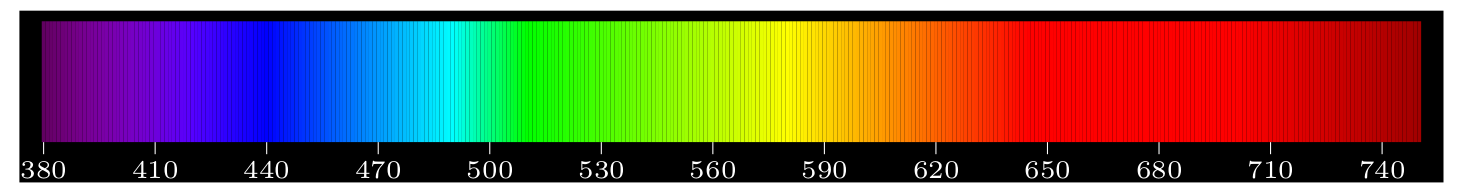
\includegraphics[width=.8\columnwidth]{img/spettrolum.png}
\end{figure}}
\end{frame}



\begin{frame}
\frametitle{Blueshift}
\begin{center}
$ z = \dfrac{f}{f'} - 1 $
\end{center}
Se sorgente e rilevatore si avvicinano, $ f' > f $ e \alert{$ z < 0 $}.\\~\pause\\
Si parla allora di \alert{blueshift}, poiché $ \lambda' < \lambda $ e la luce visibile si sposta verso il blu.

\visible<2>{\begin{figure}
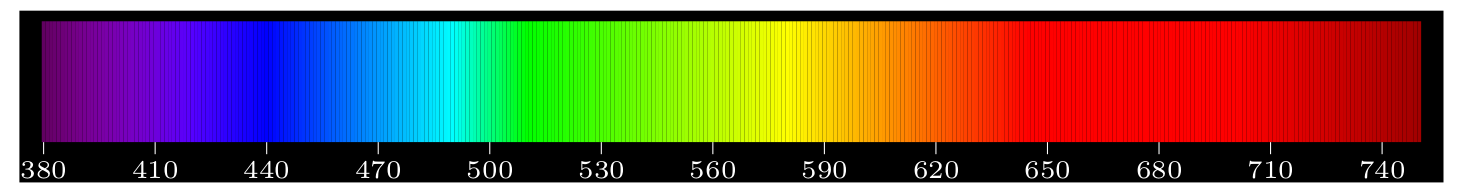
\includegraphics[width=.8\columnwidth]{img/spettrolum.png}
\end{figure}}
\end{frame}


\begin{frame}
\frametitle{Riassumendo}

\centering
  \begin{tabular}{c|c|c}
    &\textbf{Allontanamento} & \textbf{Avvicinamento} \\\hline\rule{0pt}{3ex}
    frequenza & $ f' < f $ & $ f' > f $ \\\rule{0pt}{6ex}
    lungh.~d'onda & $ \lambda' > \lambda $ & $ \lambda' < \lambda $ \\\rule{0pt}{6ex}
    formula & $ f' = f \sqrt{\frac{1 - \beta}{1 + \beta}} $ & $ f' = f \sqrt{\frac{1 + \beta}{1 - \beta}} $ \\\rule{0pt}{6ex}
    $ z = \frac{f}{f'} - 1 $ & $ z >0 $ & $ z < 0 $ \\\rule{0pt}{6ex}
    effetto & redshift & blueshift \\
  \end{tabular}
\end{frame}





\begin{frame}
\frametitle{Esercizio}
\begin{exampleblock}{Velocità di allontanamento}
\small{
  Un \emph{quasar} emette onde luminose con frequenza $ f $. La frequenza delle stesse onde misurata sulla Terra è $ f' = 0,75f $.

  Calcola la velocità di allontanamento relativo tra la Terra e il \emph{quasar}.\hspace*{\fill}[$ 8,4 \times 10^{7} \, m/s $]
  }
\end{exampleblock}

~

\begin{exampleblock}{Dalla frequenza alla lunghezza d'onda}
\small{
  Una sorgente emette luce la cui lunghezza d'onda è $ \lambda = 520 \, nm $. La sua velocità di avvicinamento alla Terra è pari a due terzi della velocità della luce nel vuoto.

  Calcola la lunghezza d'onda $ \lambda' $ rilevata da un osservatore a Terra.\hspace*{\fill}[$ 233 \, nm $]
  }
\end{exampleblock}
\end{frame}




\section{Minkowski}


\begin{frame}
  \frametitle{Intervallo invariante}
Un certo spostamento nello spazio $ \Delta\vec{s} = (\Delta x, \Delta y, \Delta z ) $ può essere descritto in diversi SDR con diverse componenti.
  
\begin{columns}
\begin{column}{0.4\textwidth}

\begin{figure}
\begin{tikzpicture}[scale=.6]
\draw [->,red] (0,0) -- (4,0);
\draw [->,red] (0,0) -- (0,4);
\draw [->,thick] (0,0) -- (1.5,3);
\draw [dashed] (1.5,3) -- (1.5,0);
\draw [dashed] (1.5,3) -- (0,3);
\node [below,red] at (4,0) {{\scriptsize $ x $}};
\node [below] at (.75,0) {{\scriptsize $ \Delta x $}};
\node [left] at (0,1.5) {{\scriptsize $ \Delta y $}};
\node [left,red] at (0,4) {{\scriptsize $ y $}};
\end{tikzpicture}
\end{figure}

\end{column}
\begin{column}{0.4\textwidth}

\begin{figure}
\begin{tikzpicture}[scale=.6]
\draw [->,cyan] (0,0) -- (3,2);
\draw [->,cyan] (0,0) -- (-2,3);
\draw [->,thick] (0,0) -- (1.5,3);
\draw [dashed] (1.5,3) -- (2.42,1.61);
\draw [dashed] (1.5,3) -- (-.92,1.38);
\node [below,cyan] at (3,2) {{\scriptsize $ x $}};
\node [below] at (1.7,1) {{\scriptsize $ \Delta X $}};
\node [left] at (-.5,.7) {{\scriptsize $ \Delta Y $}};
\node [above,cyan] at (-2,3) {{\scriptsize $ y $}};
\end{tikzpicture}
\end{figure}

\end{column}
\end{columns}

Notiamo tuttavia che la somma dei quadrati delle componenti rimane costante. Tale somma è detta \alert{intervallo invariante} e il suo quadrato vale:
\begin{center}
\colorbox{blue!30}{$ (\Delta s)^2  = (\Delta x )^2 + (\Delta y )^2 + (\Delta z )^2 $}
\end{center}
\end{frame}


\begin{frame}
\frametitle{Lo spaziotempo}
La relatività ristretta non utilizza uno spazio euclideo, ma uno spazio quadridimensionale detto \emph{spazio di Minkowski} (formulato da Hermann Minkowski nel 1907-1908) o \emph{spaziotempo}.\pause

~

In questo spazio l'intervallo invariante è definito come:
\begin{center}
\colorbox{blue!30}{$ (\Delta \sigma)^2  = (c\Delta t)^2 - (\Delta x )^2 - (\Delta y )^2 - (\Delta z )^2 $}
\end{center}\pause

~

$ \Delta \sigma $ è un quadrivettore con quattro componenti, una temporale e tre spaziali e risulta invariante se applichiamo le trasformazioni di Lorentz.

\end{frame}


\begin{frame}
\frametitle{L'intervallo invariante per diversi spazi geometrici}
\centering
  \begin{tabular}{c|c|c}
    \textbf{Spazio} & \textbf{Coord.} & \textbf{Quadrato dell'int.~invariante} \\\hline\rule{0pt}{3ex}
    Euclideo 2D & $ x,y $ & $ (\Delta s)^2  = (\Delta x )^2 + (\Delta y )^2 $ \\\rule{0pt}{6ex}
    Euclideo 3D & $ x,y,x $ & $ (\Delta s)^2  = (\Delta x )^2 + (\Delta y )^2 + (\Delta z )^2 $ \\\rule{0pt}{6ex}
    Spaziotempo 2D & $ t,x $ & $ (\Delta \sigma)^2  = (c\Delta t)^2 - (\Delta x )^2 $ \\\rule{0pt}{6ex}
    Spaziotempo 4D & $ t,x,y,z $ & $ (\Delta \sigma)^2  = (c\Delta t)^2 - (\Delta s )^2 $ \\
  \end{tabular}
\end{frame}


\begin{frame}
\frametitle{Diagrammi di Minkowski (2)}
Scegliamo eventi che si trovano allineati lungo l’asse $ x $, con proporzioni opportune.
\begin{figure}
\begin{tikzpicture}[xscale=.4,yscale=.4]
\draw [->] (-.5,0) -- (8,0);
\draw [->] (0,-.5) -- (0,8);
\draw[smooth, orange, thick, domain=0:6, samples=50] plot 
({\x},{  \x });
\draw[smooth, olive, thick, domain=0:2.5, samples=50] plot 
({\x},{ 2* \x });
\draw [thick, red] (0,0) -- (0,7);
\node [right, red] at (0,7) {{\tiny corpo fermo}};
\node [above, olive] at (2.5,5) {{\tiny corpo in MRU}};
\node [above, orange] at (6,6) {{\tiny segnale luminoso}};
\node [below] at (1,0) {{\tiny $ 1 $}};
\node [below] at (2,0) {{\tiny $ 2 $}};
\node [below] at (3,0) {{\tiny $ 3 $}};
\node [below] at (4,0) {{\tiny $ 4 $}};
\node [below] at (5,0) {{\tiny $ 5 $}};
\node [below] at (6,0) {{\tiny $ 6 $}};
\node [below] at (9,0) {{\tiny $ x \, \left[ \times 10^8 \, m \right] $}};
\node [left] at (0,1) {{\tiny $ 1 $}};
\node [left] at (0,2) {{\tiny $ 2 $}};
\node [left] at (0,3) {{\tiny $ 3 $}};
\node [left] at (0,4) {{\tiny $ 4 $}};
\node [left] at (0,5) {{\tiny $ 5 $}};
\node [left] at (0,6) {{\tiny $ 6 $}};
\node [left] at (0,8) {{\tiny $ t [s] $}};
\end{tikzpicture}
\end{figure}
Le TdL permettono di passare da un SDR ad un altro lasciando invariate le \emph{linee di universo} di c. \href{https://www.youtube.com/watch?v=Rh0pYtQG5wI}{\beamergotobutton{Trasformazioni di Lorentz e shearing}}
\end{frame}




\begin{frame}
\frametitle{Diagrammi di Minkowski}
\begin{figure}
\begin{tikzpicture}[xscale=.4,yscale=.4]
\draw [->] (-8,0) -- (8,0);
\draw [->] (0,-8) -- (0,8);
\angolo[<->, dashed, teal](0,0)(45:135:3)
\node [above, teal] at (-1.7,3) {{\tiny moti possibili}};
\node [right, violet] at (3,1) {{\tiny moti impossibili}};
\node [right, cyan] at (0,7) {{\tiny futuro}};
\node [right, cyan] at (0,-7) {{\tiny passato}};
\angolo[<->, dashed, violet](0,0)(-45:45:3)
\draw[smooth, orange, thick, domain=-5:5, samples=50] plot 
({\x},{  \x });
\draw[smooth, orange, thick, domain=-5:5, samples=50] plot 
({\x},{ -\x });
\node [above, orange] at (5,5) {{\tiny cono di luce}};
\node [below] at (9,0) {{\tiny $ x \, \left[ \times 10^8 \, m \right] $}};
\node [left] at (0,8) {{\tiny $ t [s] $}};
\end{tikzpicture}
\end{figure}
\end{frame}


\begin{frame}
\frametitle{Minkowski 3D}
\begin{figure}
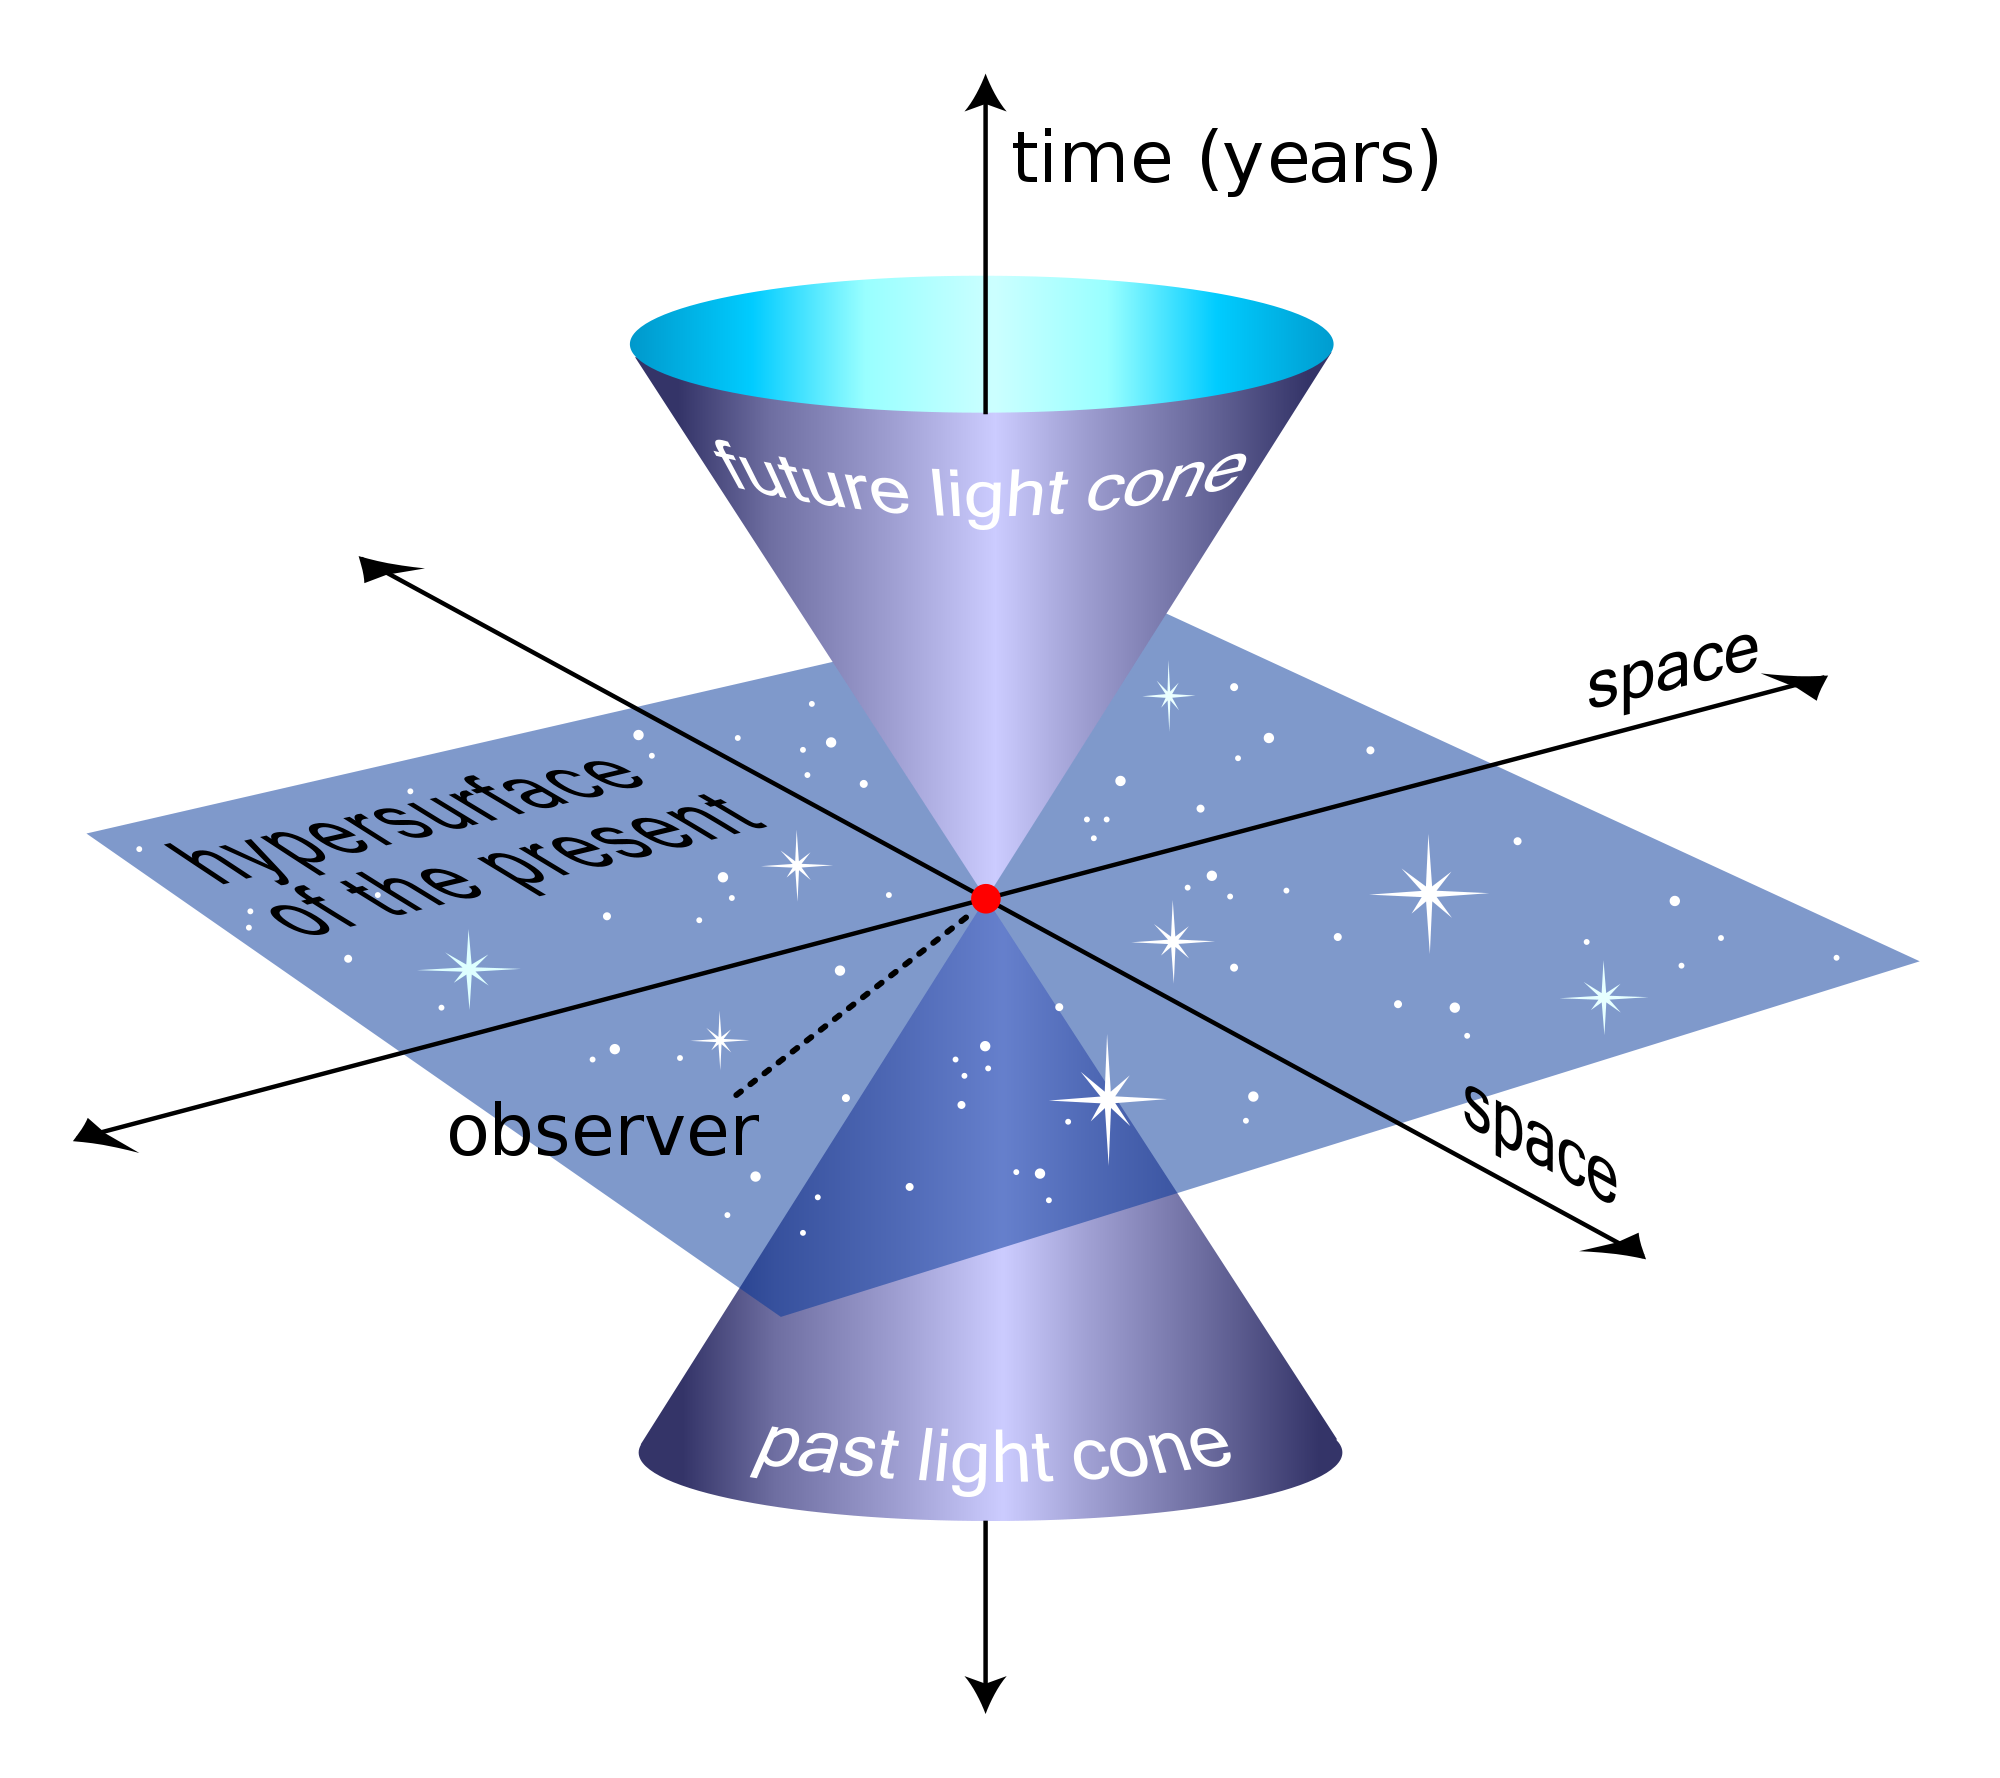
\includegraphics[width=.8\columnwidth]{img/minkowski.png}
\end{figure}
\end{frame}


\begin{frame}
\frametitle{Causalità}
Possiamo individuare tre regioni in un diagramma di Minkowski:
\begin{itemize}
  \item una regione \alert<1>{accessibile dal qui e ora}, all'interno del cono di luce, in cui sono ammesse interazioni causali col qui e ora;\pause
  
\begin{center}
    \alert<2>{$ (\Delta \sigma)^2 > 0 $}, intervallo di tipo tempo.
  \end{center}\pause
  \item una regione \alert<3>{accessibile dal qui e ora solo con un'onda luminosa}, il cono di luce, in cui le interazioni causali possono avvenire solo tramite onde elettromagnetiche;\pause
  
\begin{center}
    \alert<4>{$ (\Delta \sigma)^2 = 0 $}, intervallo di tipo luce.
  \end{center}\pause
  \item una regione \alert<5>{inaccessibile dal qui e ora}, all'esterno del cono di luce, causalmente indipendente dal qui e ora.\pause
    
\begin{center}
    \alert<6>{$ (\Delta \sigma)^2 < 0 $}, intervallo di tipo spazio.
  \end{center}
\end{itemize}
\end{frame}

\section{Dinamica}

\begin{frame}
\frametitle{Massa relativistica (1)}
Secondo la dinamica classica dovrebbe essere possibile applicare una forza per un tempo sufficientemente lungo (ma non infinito) ad un corpo per fargli superare $ c $\footnote{Vedi il \emph{teorema dell'impulso}: $ F \Delta t = m \Delta v $.}.\pause

~

In relatività, l'idea è che l'inerzia di un corpo (la sua resistenza al moto) dipenda dal suo contenuto energetico.\pause

~

Definiamo la \alert{massa relativistica}:
\begin{center}
\colorbox{blue!30}{$ m = \gamma m_0 $}
\end{center}
dove $ m_0 $ è la massa del corpo a riposo, misurata in un SDR in cui il corpo è in quiete.
\end{frame}

\begin{frame}
\frametitle{Massa relativistica (2)}
In effetti, vediamo che:
\begin{center}
$ \displaystyle \lim_{v \to c} \gamma m_0 = + \infty $
\end{center}
Per accelerare un tale corpo sarebbe necessaria una quantità infinita di energia.\pause

~

I valori di $ m $ e di $ m_0 $ diventano significativamente diversi per velocità oltre i $ 60 $ milioni di metri al secondo.
\end{frame}

\begin{frame}
\frametitle{Variazione di massa}
Da quanto detto, risulta che se un corpo riceve un'energia $ E $ la sua massa non si conserva, ma aumenta della quantità:
\begin{center}
$ \Delta m = \dfrac{E}{c^2} $
\end{center}
Viceversa, la massa di un corpo diminuisce se esso perde energia.
\end{frame}


\begin{frame}
\frametitle{Energia a riposo}
In relatività risulta allora che la massa non è altro che una forma di energia. Detto altrimenti, un corpo possiede una certa quantità di energia per il solo fatto di avere una massa.\pause

~

Definiamo allora l'\alert{energia a riposo} di un corpo come:
\begin{center}
\colorbox{blue!30}{$ E_0 = m_0 c^2  $}
\end{center}
\end{frame}


\begin{frame}
\frametitle{Energia cinetica relativistica}
Un corpo in movimento possiede, secondo la meccanica relativistica, anche una certa \alert{energia cinetica relativistica}:
\begin{center}
\colorbox{blue!30}{$ E_C = (\gamma - 1) m_0 c^2 $}
\end{center}\pause

~

Tale energia cinetica si riduce alla già nota $ E_C = \dfrac{1}{2}mv^2 $ per velocità molto inferiori a $ c $.
\end{frame}


\begin{frame}
\frametitle{La relazione di Einstein}
Un corpo avrà quindi un'energia totale data dalla somma tra la sua energia cinetica e la sua energia a riposo:
\begin{center}
$ E = E_C + E_0 = (\gamma - 1) m_0 c^2 + m_0 c^2 = (\gamma m_0) c^2  $
\end{center}\pause
da cui, ricordando che $ m = \gamma m_0 $:
\begin{center}
\colorbox{blue!30}{$ E = m c^2  $}

~

\href{http://tinyurl.com/y44pmj7w}{\beamergotobutton{Tomografia a emissione di positroni}}
\end{center}
\end{frame}



\begin{frame}
\frametitle{La quantità di moto relativistica}
Possiamo anche definire una \emph{quantità di moto relativistica}, che si riduce a quella classica a basse velocità:
\begin{center}
\colorbox{blue!30}{$ \vec{p} = m \vec{v} = \gamma m_0 \vec{v}  $}
\end{center}\pause

~

Ricordiamo che la quantità di moto è una quantità vettoriale, che avrà tre dimensioni spaziali nello spazio di Minkowski.
\end{frame}







\begin{frame}
\frametitle{Esercizi}
\begin{exampleblock}{Energia e quantità di moto relativistiche (1)}
\small{
Una particella relativistica è accelerata fino ad acquistare un'energia totale di $ 6,45 \times 10^{-8} \, J $ e una quantità di moto di $ 21,3 \times 10^{-17} \, kg \cdot m/s $.

Calcola la velocità finale della particella.\hspace*{\fill}[$ 2,97 \times 10^{8} \, m/s $]
  }
\end{exampleblock}

~

\begin{exampleblock}{Energia e quantità di moto relativistiche (2)}
\small{
Una particella che viaggia alla velocità di $ 8,0 \times 10^{7} \, m/s $ è accelerata e la sua quantità di moto diventa il doppio di quella iniziale.

Calcola la velocità finale della particella.\hspace*{\fill}[$ 1,5 \times 10^{8} \, m/s $]
  }
\end{exampleblock}
\end{frame}



\begin{frame}
\frametitle{Il quadrivettore energia-quantità di moto (1)}
Per un corpo con energia totale $ E $ e in moto a velocità $ \vec{v} $, definiamo un vettore a quattro componenti con le dimensioni della quantità di moto:
\begin{center}
\colorbox{blue!30}{$ \left( \dfrac{E}{c} , p_x , p_y , p_z \right) $}
\end{center}
\end{frame}

\begin{frame}
\frametitle{Il quadrivettore energia-quantità di moto (2)}
Supponiamo per semplicità che $ \vec{v} $ abbia solo componente lungo l'asse $ x $, e pertanto il quadrivettore sarà:
\begin{center}
$ \left( \dfrac{E}{c} , p , 0 , 0 \right) $
\end{center}\pause

~

Calcoliamo il quadrato del modulo di tale vettore, ricordando che ci troviamo in un spazio di Minkowski.
\begin{center}
$ \left( \dfrac{E}{c} \right)^2 - p^2 = \left(\dfrac{\gamma m_0 c^2}{c}\right)^2 - (\gamma m_0 v)^2 = \left(\gamma m_0 c\right)^2 - (\gamma m_0 v)^2 $
\end{center}
\end{frame}

\begin{frame}
\frametitle{Il quadrivettore energia-quantità di moto (3)}
\begin{center}
$ \gamma^2 m_0^2 (c^2 - v^2) = \dfrac{1}{~~\frac{c^2 - v^2}{c^2}~~} m_0^2 (c^2 - v^2) = \dfrac{c^2}{~~\cancel{c^2 - v^2}~~} m_0^2 (\cancel{c^2 - v^2})$
\end{center}\pause
da cui:
\begin{center}
\colorbox{blue!30}{$ \left( \dfrac{E}{c} \right)^2 - p^2 = m_0^2 c^2  $}
\end{center}\pause

\alert{Il modulo di questo vettore risulta quindi un invariante nello spazio di Minkowski}, in quanto prodotto di due invarianti.
\end{frame}




\end{document}
